\documentclass[fleqn,10pt]{wlscirep}
\usepackage[utf8]{inputenc}
\usepackage[T1]{fontenc}
\usepackage{bm}
\title{Variation in Normalized Difference Vegetation Index in canola paddock during in a growing season}
\author[1,*]{Germán Eduardo González González}
\begin{document}
\flushbottom
\maketitle 
Despite the success of canola in Australian cropping systems, significant gaps remain in the underlying knowledge of canola physiology and agronomy, a situation exacerbated by its expansion into new areas and the release of new technologies. The evolution of the cultivation of Canola depends on multiple variables such as the weather, the intensity of the sun, water, and other variables that help the plants grow healthily. The best way to estimate the state of the plant is using the normalized difference vegetation index (NDVI), which uses remote sensing to evaluate light absorption during the photosynthesis process and detect abnormal changes in its growth.
\\~\\
This document shows the procedure to estimate a time series of NDVI for any area in the world and explain how to interpret and visualize this index to help to make more informed decisions about the cultivation. We use this method in one Canola paddock in NSW (Australia) and estimate the time series of NDVI for the 2021 growing season that extends from April 1 to October 1. Finally, this document recommends that the project should invest further in remote sensing technology to understand the circumstance that affects the cultivation and optimize the production of this canola paddock.
\\~\\
Firstly, regarding NDVI, this index is a measure of vegetation greenness (Joran 1969, Tucker 1979) that is calculated from the visible and near-infrared light (NIR) reflected by vegetation. The estimation uses a satellite image from different bands of spectrum, and uses this equation: $ NDVI =(NIR-Red)/(NIR+Red) $. The intuition of this equation is that the Healthy vegetation (chlorophyll) absorbs most of the visible light and reflects a large portion of the near-infrared light. Otherwise, unhealthy vegetation reflects more visible light and less near-infrared light. The result of this formula generates a value between -1 and +1. If the plant has a low reflectance in the red channel and high reflectance in the NIR channel, this will get an NDVI value and vice versa. The image below shows the relationship between the NDVI and the state of the plant.
\begin{center}
\captionsetup{type=figure}
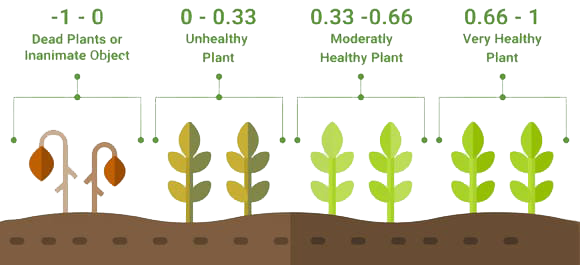
\includegraphics[width=0.38\linewidth]{scale.png}
\captionof{figure}{Interpretation of the NDVI.}
\label{fig:esquema_general}
\end{center}
After understanding how to calculate the NDVI, it is important to understand how to obtain the images inputs. The source of information is very important to building the NDVI, where each satellite has parameters and calibration of NIR and red spectrum. Depending on the use of NDVI the source of information could be changed. Each satellite has different features and performance, and some of the main features that consider building a time series of NDVI is the resolution and the time to have the available data (repeat cycle of the surface). The table below shows three of the main features for satellites available and the number of values of NDVI that could be estimated between April 1 to October 1 in the Canola paddock study case (N-timeserie).  
\begin{table}[]
\centering
\begin{tabular}{ccccc}
\hline
\textbf{Satellite} & \textbf{Cycle of recollection} & \textbf{Resolution} & \textbf{Launched} & \textbf{N-Timeserie} \\
\hline
Pleiades           & 26 days                        & 50 cm                & 2/12/12           & 7                    \\
Landsat 8          & 16 days                        & 30 m                & 11/2/13           & 12                   \\
Sentinel 2         & 10 day                         & 10 m                & 23/6/15           & 18                  
\\ 
\hline
\end{tabular}
\caption{Sources Features} 
\label{table:ventanasminutos}
\end{table}
In this study, we choose Sentinel 2 because it combines good resolution and permits the creation of the largest time series (18 values) in comparison to other satellites. On this point it is important to mention that there exists a trade-off between the cycle of days and the bias. For example, the Pleiades satellite has the best resolution (less bias) but the values that we estimate are the lowest. This study prefers the largest time series with a slight bias to analyse the evolution of the canola during the growing season.
\\~\\ 
After choosing the source of information, we collect this data through Google Earth Engine (GEE). We chose this platform because it combines geospatial analysis tools in Python with GEE, and it permits getting information in a particular area at any moment of time.  The procurement that we do to estimate the NDVI is: 
\begin{itemize}
\setlength\itemsep{0em}
\item Choose the paddock with centroid: latitude -34.835395 and longitude 149.677364.
\item Create polygon: circumference with a radio of 500 around the centroid
\item Create a time grid between April 1 to October 1 of 2021 every two weeks.
\item Get the images from Sentinel 2 from the polygon area for each interval date in the grid.
\item Calculate the average NDVI in the area covered by the polygon. 
\item Interpolation with splines two dates that were a cloudy day and do not have data of the NIR
\item Create the NDVI Map for each interval date in the grid
\end{itemize}
\begin{figure}[!h]
\centering
\begin{minipage}[b]{0.6\textwidth}
\centering
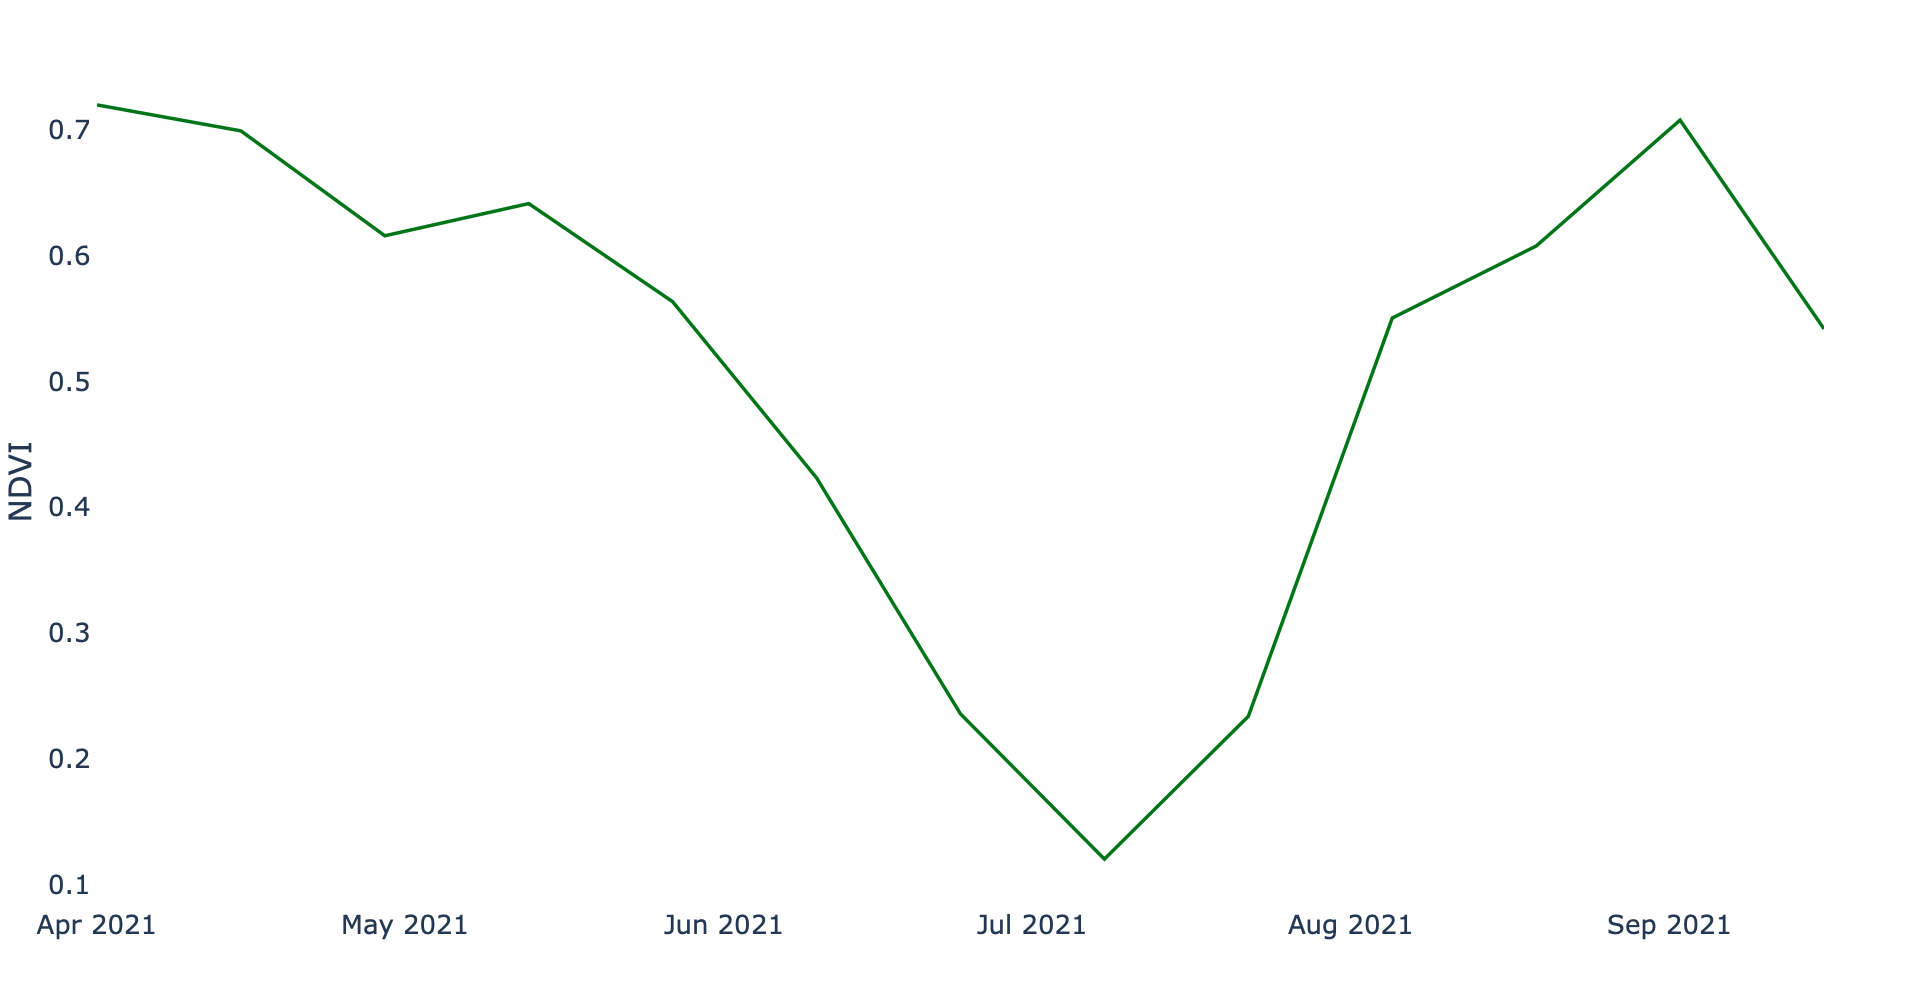
\includegraphics[width=\textwidth]{time.png}
\caption{NDVI: April 1 to October 1.}
\end{minipage}
\hfill
\begin{minipage}[b]{0.35\textwidth}
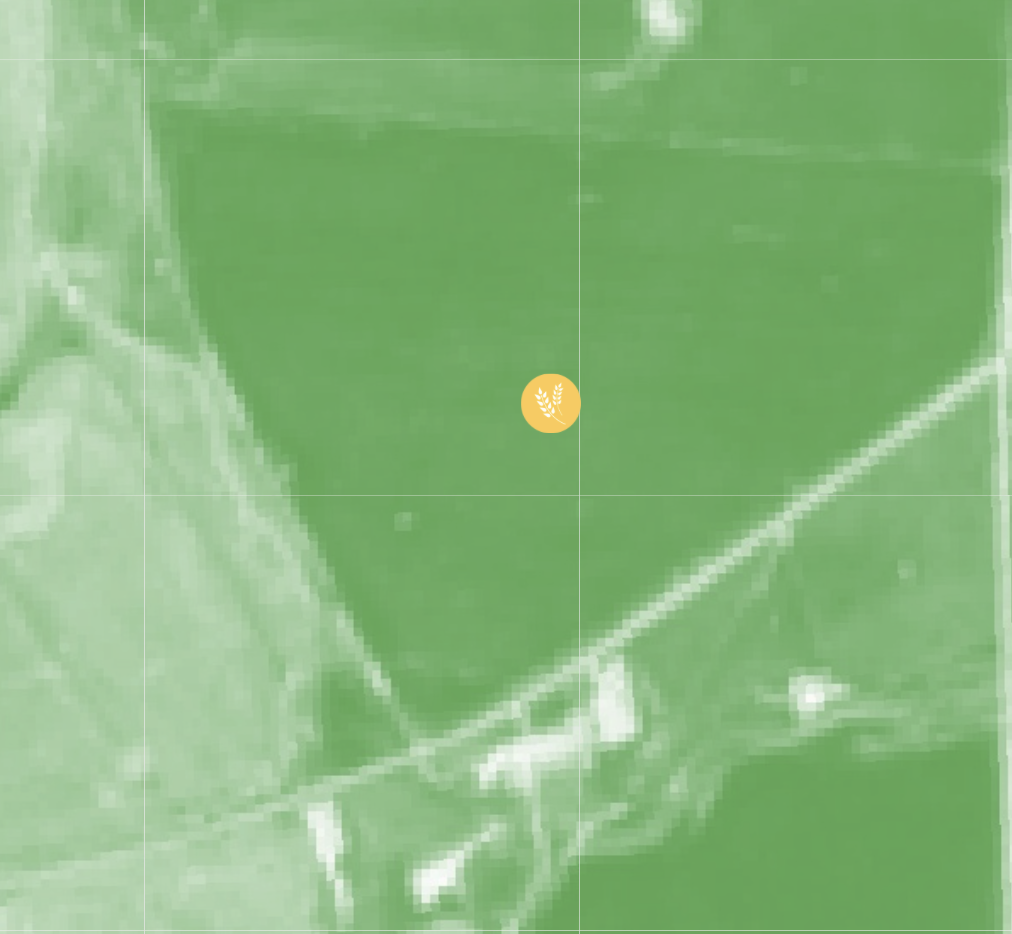
\includegraphics[width=\textwidth]{crop.png}
\caption{NDVI in the cover area.}
\end{minipage}
\end{figure}
In the picture, it is evident a correlation between NDVI and the season effect. The table below shows the main insights about the time series and the state of the plant in each season: 
\begin{table}[h]
\centering
\begin{tabular}{cccc}
\hline
\textbf{Season} & \textbf{Period}                & \textbf{Range}     & \textbf{NDVI - Average state} 
\\
Autumn & April and May         & 0.5 - 0.7 & Very healthy plant   \\
Winter & June to August        & 0.2 - 0.6 & Unhealthy plant      \\
Spring & September to November & 0.5 - 0.7 & Very healthy plant 
\\
\hline
\end{tabular}
\caption{Insights} 
\label{table:ventanasminutos}
\end{table}
\\
In addition, the NDVI calculated in the paddock is uniform around the area, which means that the territory does not have imperfections or irrigation problems. Although the results of this procedure to estimate the NDVI is stable in this area, we recommend that to improve the accuracy and depth of the study, the client invests in remote sensing technology on their project. Some of the improvements should be: 
\begin{itemize}
\setlength\itemsep{0em}
\item Connect with a private satellite that permits getting information with more resolution and frequency. 
\item Use drone and fieldwork that permits recollecting data to create a supervised model such as geospatial regression to understand which other factors are affecting the area of study.  
\item Create lead indicators and a dashboard that permits management and make more informed decisions about a number of inputs and techniques that the client should use in this area. 
\item Recollect and store this data to create analytics models that permit creation of simulated scenarios to estimate the production and the best time to crop in this paddock. 
\end{itemize}
In conclusion, the NDVI is the first approximation to create a complex GIS system that helps to control the uncertainty in agriculture in order to make an informed decision. In this study, we create a \href{https://ndvi.proactivepreventionplatform.com}{dashboard} that permits the user to interact with NDVI in each period of the timeline. 
\end{document}